%%%%%
%%%%% Supporting material for Sandwich paper.
%%%%% Compile with pdflatex as figures are not eps.
%%%%%
\documentclass[12pt,twoside]{article}
\usepackage{graphicx,color}

\setlength{\hoffset}{-1in}
\setlength{\voffset}{-1in}

\setlength{\topmargin}{2cm}
\setlength{\evensidemargin}{3.1cm}
\setlength{\oddsidemargin}{3.1cm}

\setlength{\textwidth}{14.8cm}
\setlength{\textheight}{23cm}

\setlength{\parindent}{0pt}
\setlength{\parskip}{\medskipamount}
\pagestyle{empty}

% Prepend ``Supplementary'' Fig/Table caption headings
\usepackage{caption}
\captionsetup[table]{name=Supplementary Table}
\captionsetup[figure]{name=Supplementary Figure}

% Likewise...
\renewcommand\refname{Supplementary References}

\begin{document}



{\bf Supplementary Figures}

\begin{figure}[!h]
\begin{center}
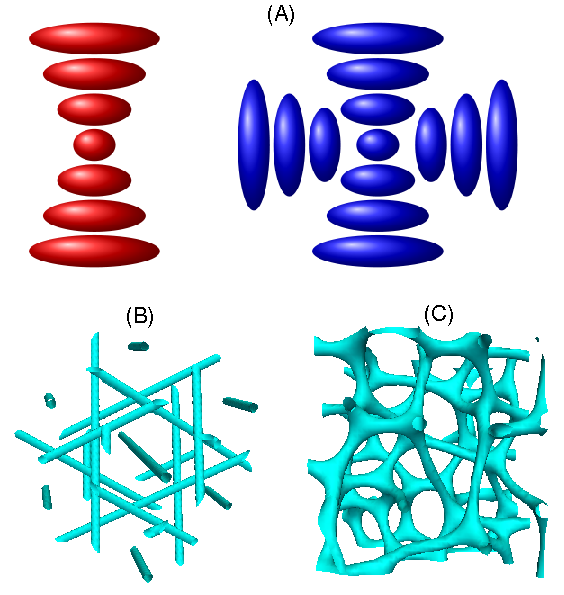
\includegraphics[scale=0.8]{support-fig1.png}
\end{center}
\caption{\textbf{Blue phase structures.}
(A) Schematic representation of the director field
in a cholesteric (left) and within a double twist cylinder (right).
(B) Snapshot of the disclination network in an equilibrated 
blue phase I structure. (C) Same as (B) for an amorphous blue phase III
network.}
\end{figure}

\newpage

\begin{figure}[!h]
\begin{center}
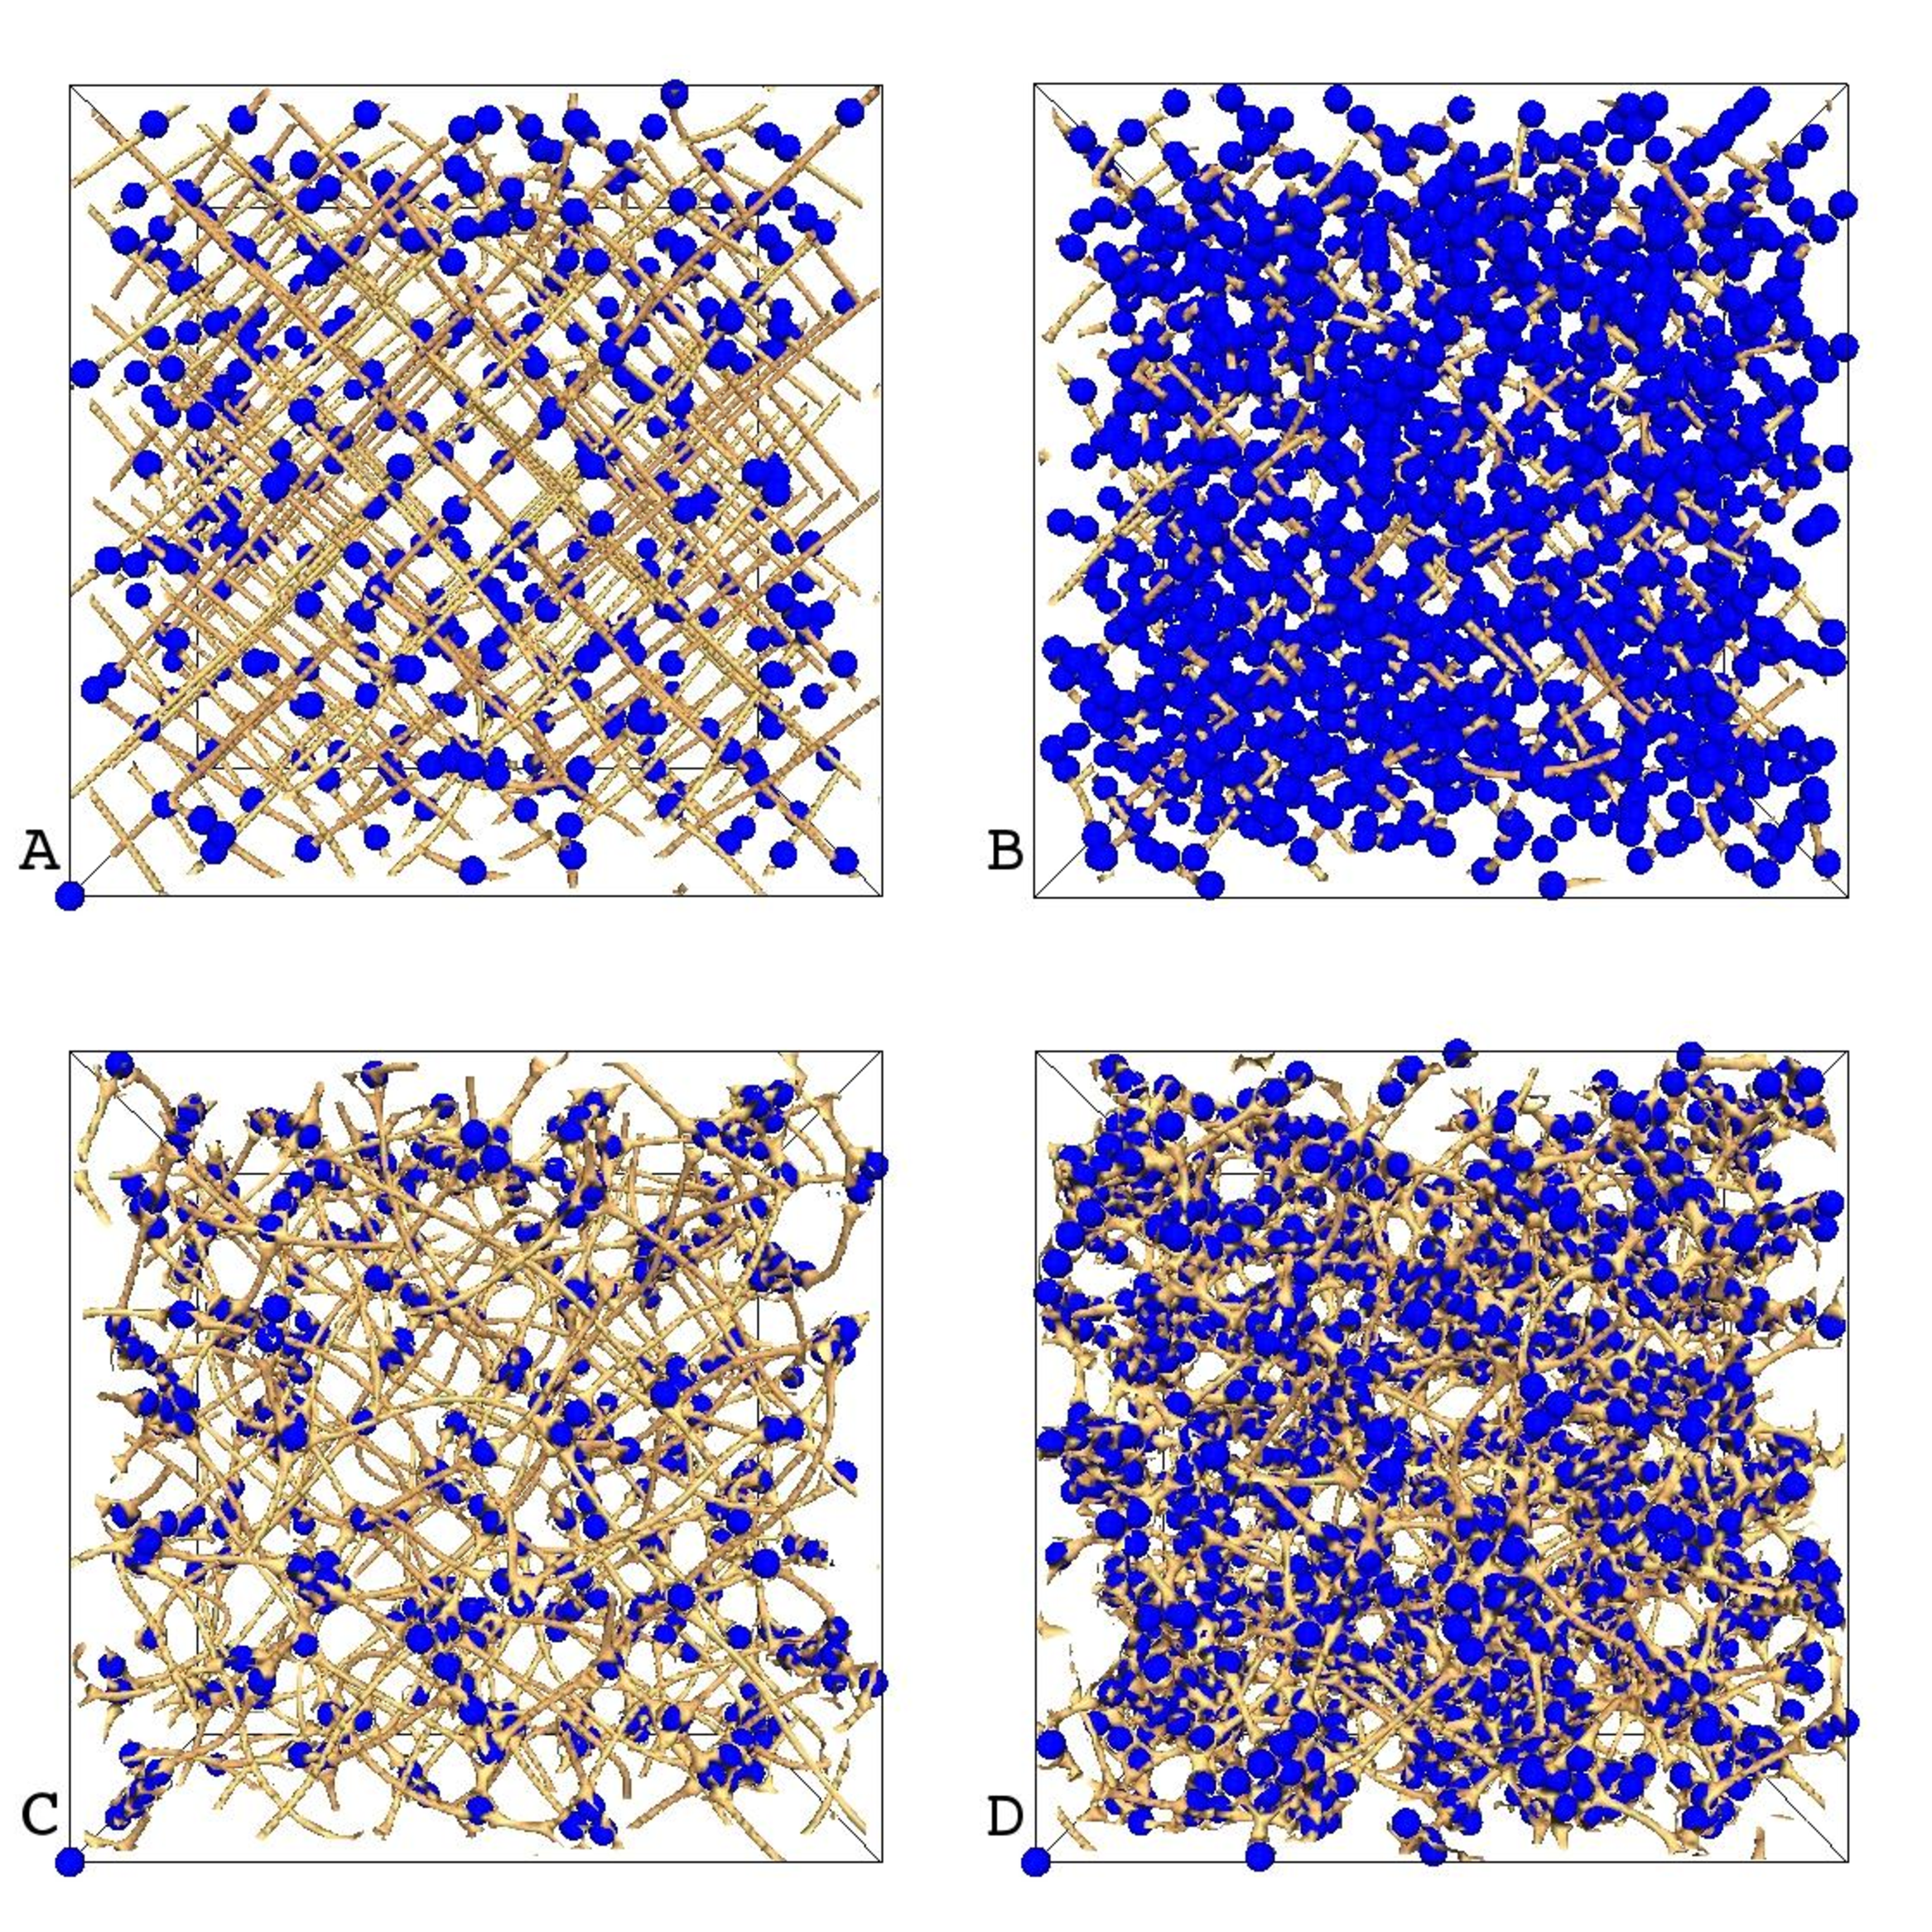
\includegraphics[scale=0.35]{support-fig2.pdf}
\end{center}
\caption{\textbf{Bulk blue phase structures.}
As for main manuscript Fig.~1 A--D
(with liquid crystal order parameter
initialised to equilibrium blue phase I structure), but for the entire
simulation system of 128$^3$ lattice sites. (A)  solid volume fraction~1\%
and weak anchoring;  (B) 4\% solid volume fraction and weak anchoring;
(C) 1\% solid volume fraction and strong anchoring; (D) 4\% solid
volume fraction and strong anchoring. The view direction in the
main figure is from the left here. There is a reference
particle at the bottom left in each panel which does not take part
in the simulation.}
\end{figure}

\newpage

\begin{figure}[!h]
\begin{center}
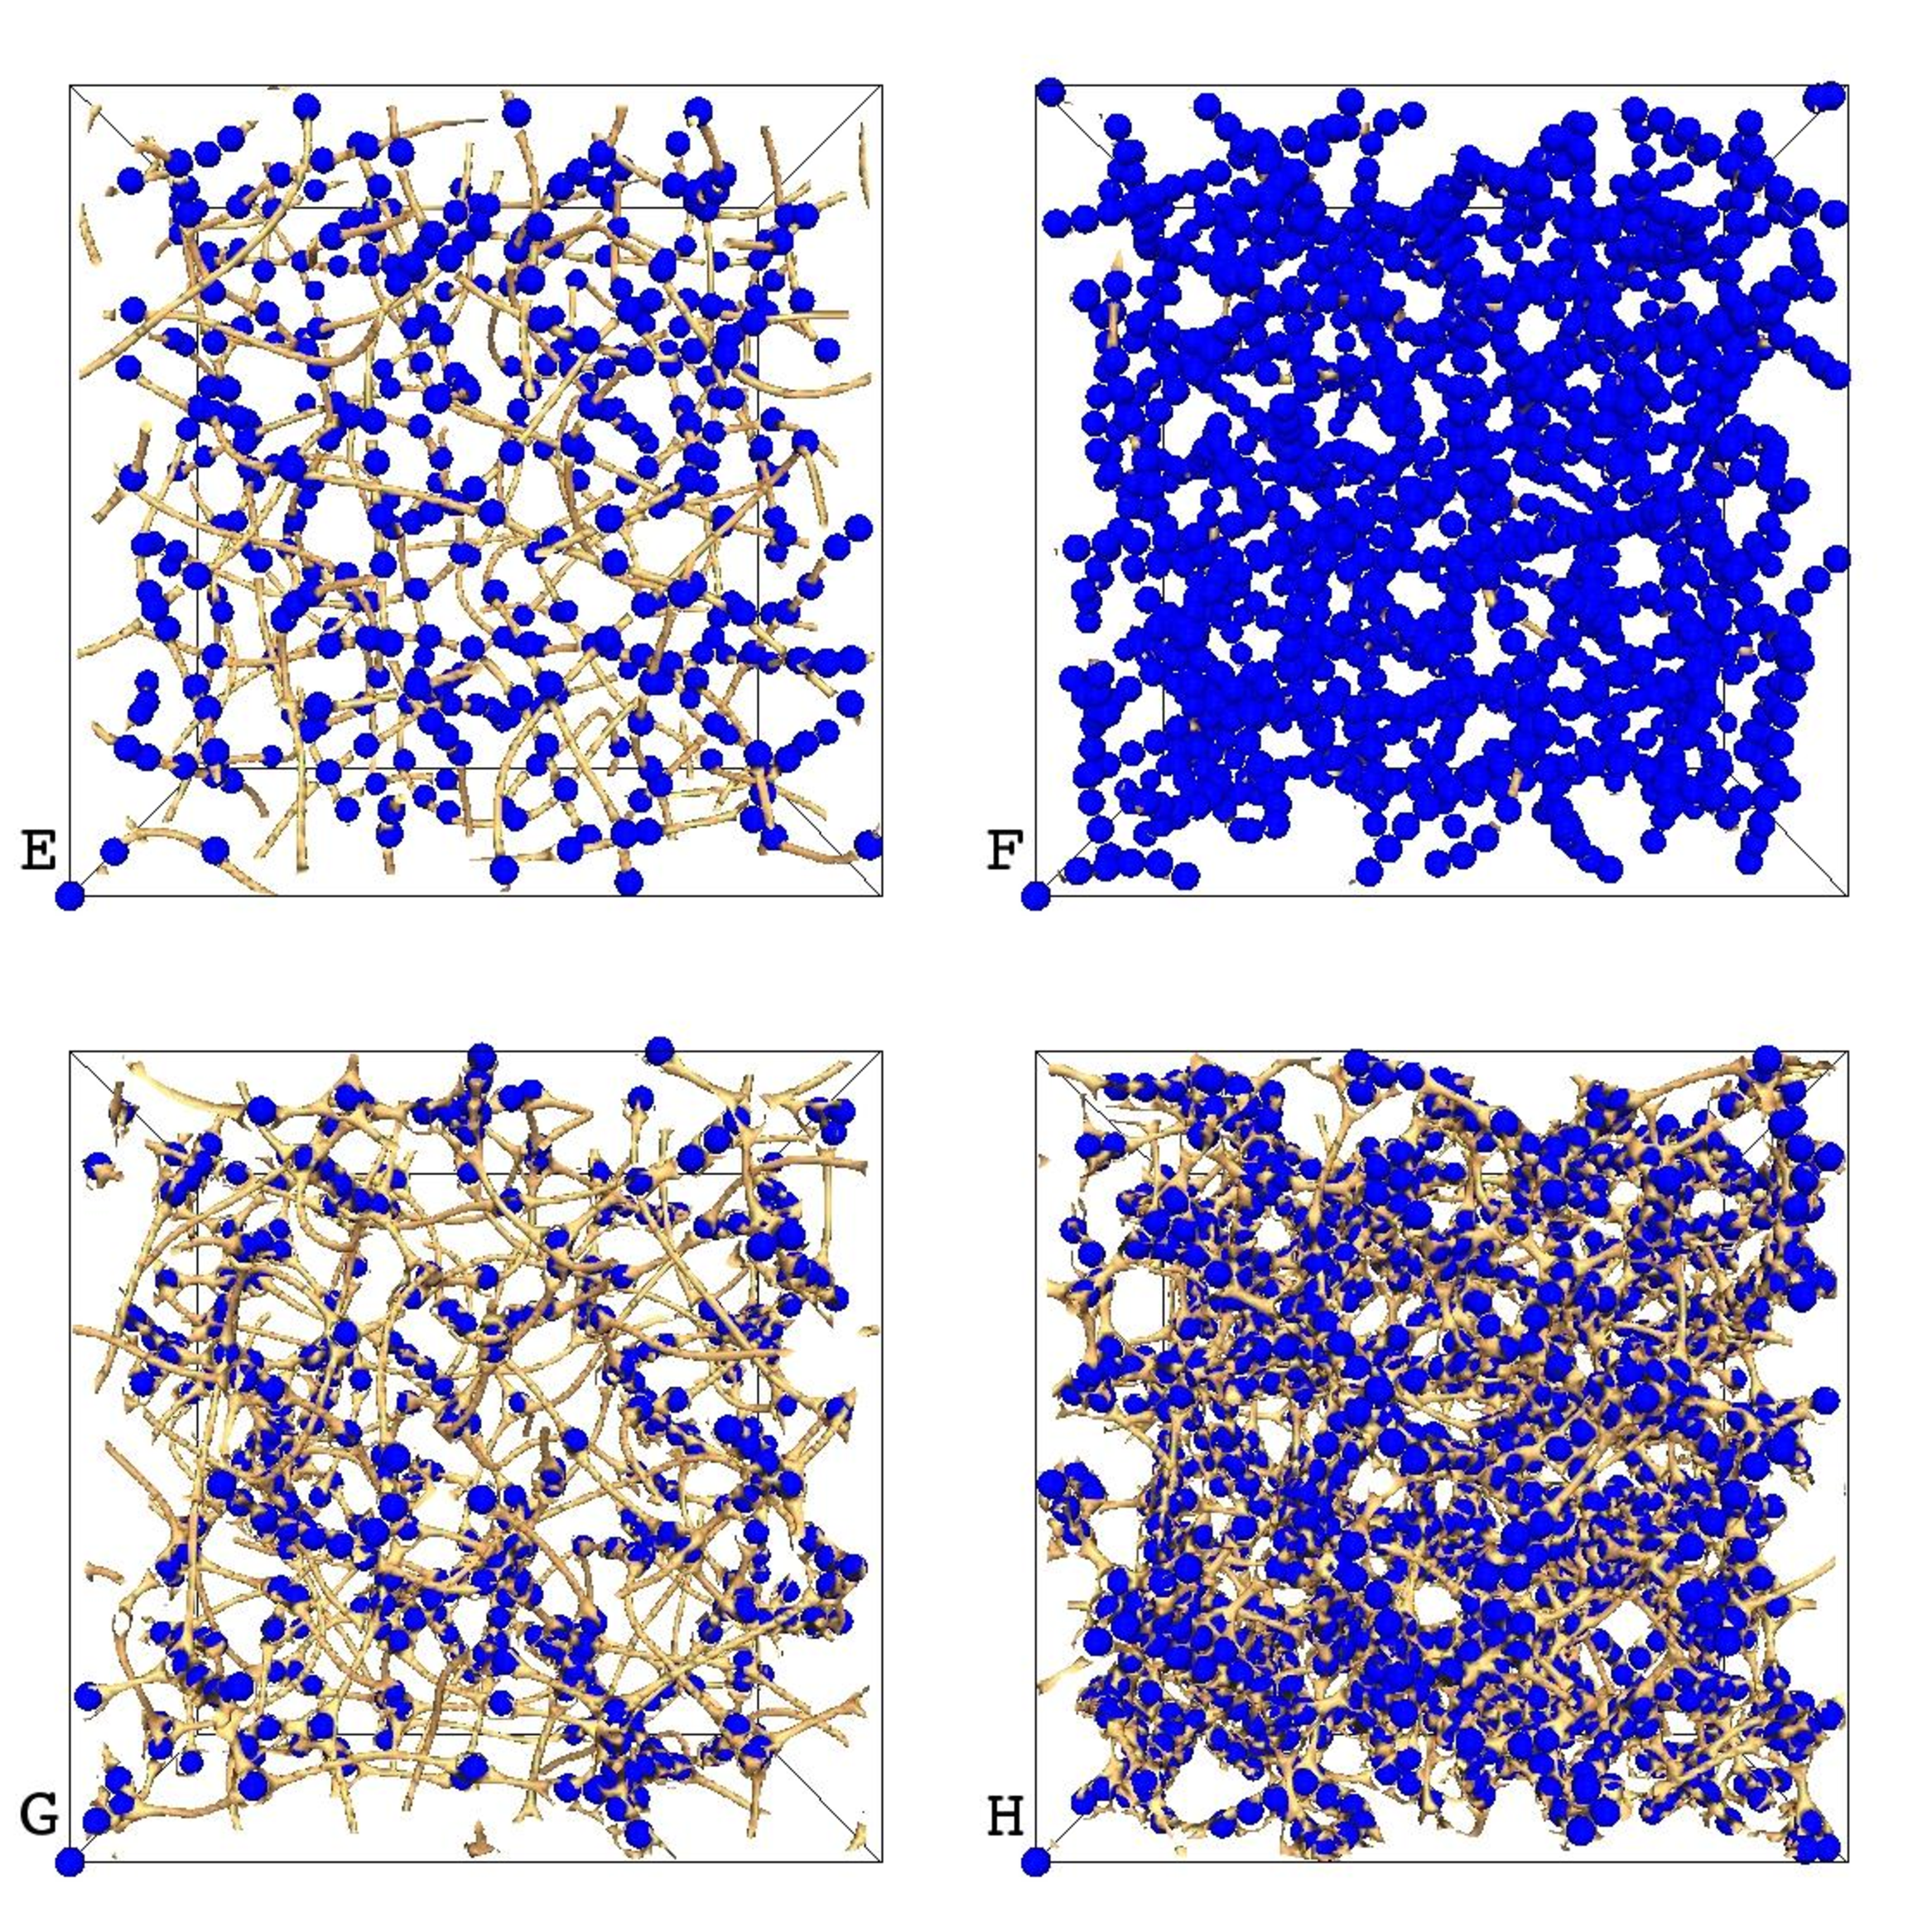
\includegraphics[scale=0.35]{support-fig3.pdf}
\end{center}
\caption{\textbf{Bulk blue phase structures.}
As for main manuscript Fig.~1 E--H (initialised via a ``quench''
to generate a disordered network), but for the entire simulation
system of 128$^3$ lattice sites. (E) solid volume fraction 1\% and
weak anchoring; (F) 4\% solid volume fraction and weak anchoring;
(G) 1\% solid volume fraction and strong anchoring; (H) 4\% solid
volume fraction and strong anchoring. Again, there is a reference
particle at the bottom left in each case which does not take part
in the simulation.}
\end{figure}

\newpage

\begin{figure}[!h]
\begin{center}
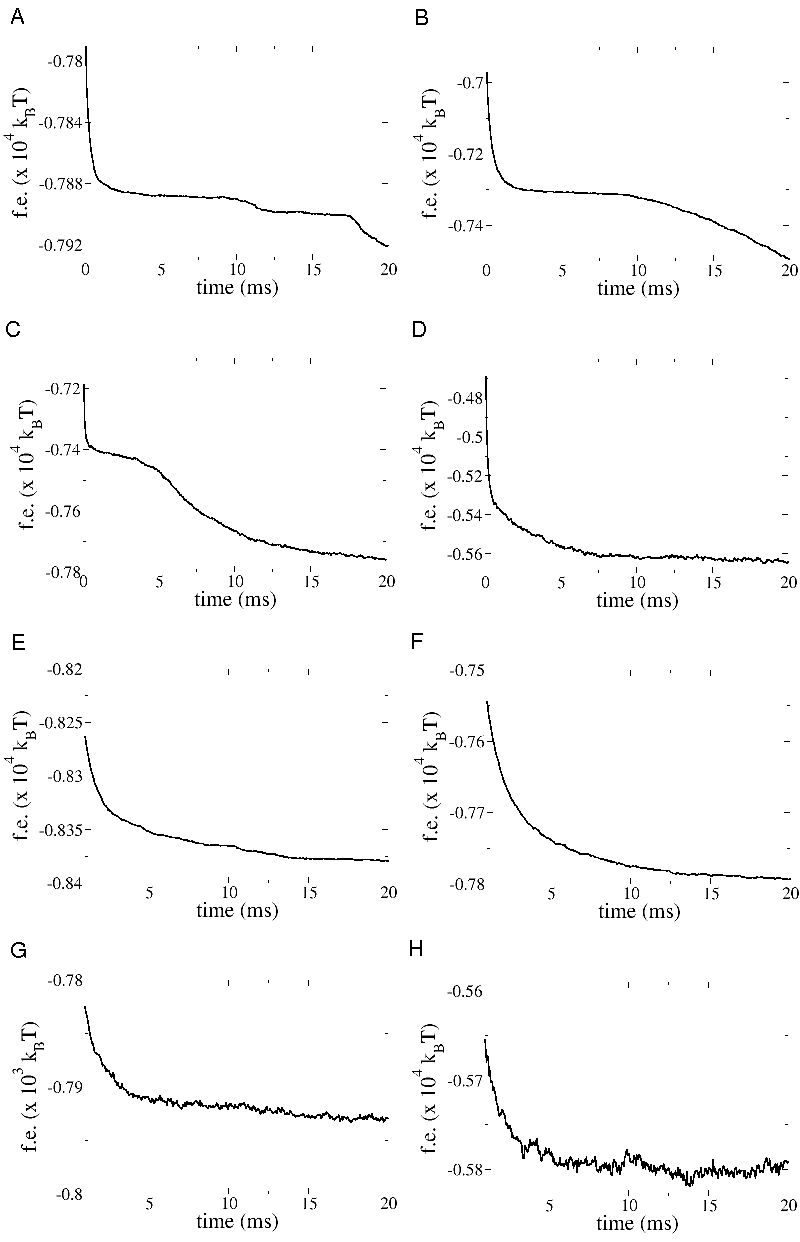
\includegraphics[scale=0.49]{support-fig4.png}
\end{center}
\caption{\textbf{Free energy evolution.}
Plot of the free energy (per BP unit cell) versus time
for the simulations corresponding to Fig. 1A-H in the main text
(the labels correspond to those in Fig. 1).
}
\end{figure}

\newpage

\begin{figure}[!h]
\begin{center}
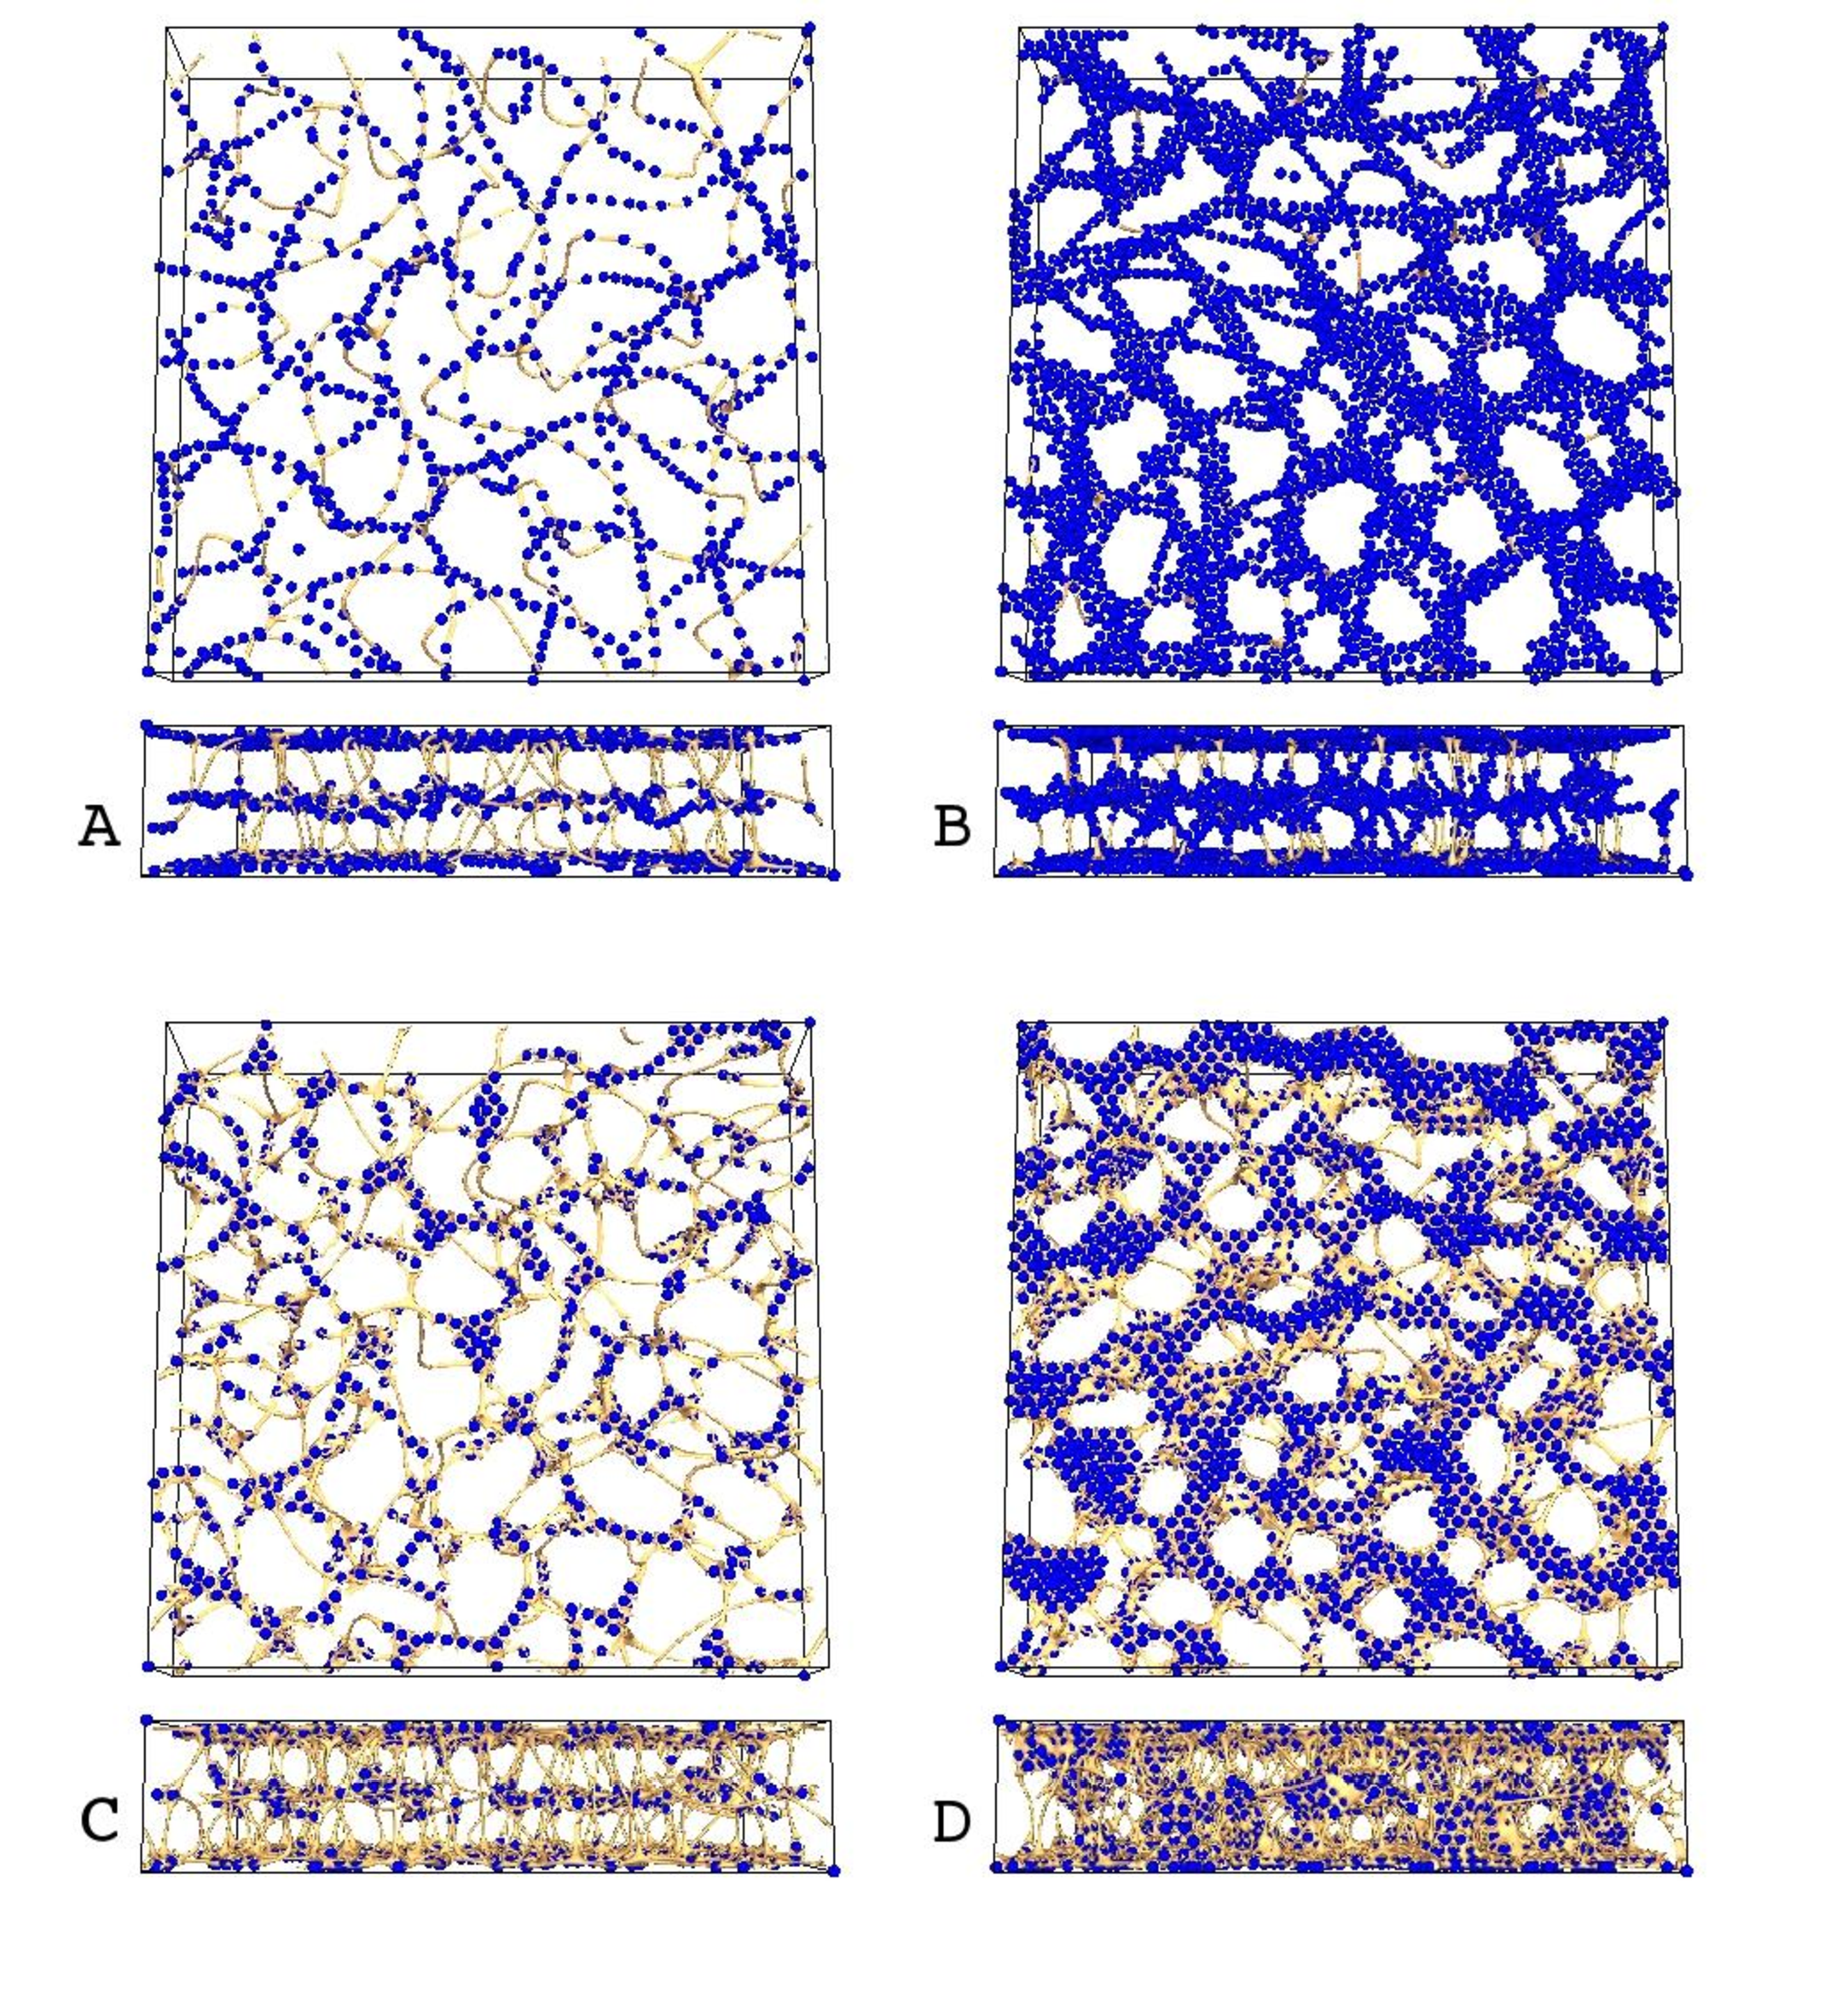
\includegraphics[scale=0.42]{support-fig5.pdf}
\end{center}
\caption{\textbf{Confined blue phase structures.}
As for main manuscript Fig.~2 A--D (confined geometry with normal
anchoring walls at both top and bottom), but for the entire simulation
system of 256$^2\times$56 lattice sites. Each shows a top view and
side view of the same simulation state. (A) solid volume fraction 1\%
and weak anchoring; (B) 4\% solid volume fraction and weak anchoring;
(C) 1\% solid volume fraction and strong anchoring; (D) 4\% solid
volume fraction and strong anchoring.}
\end{figure}

\newpage

\begin{figure}[!h]
\begin{center}
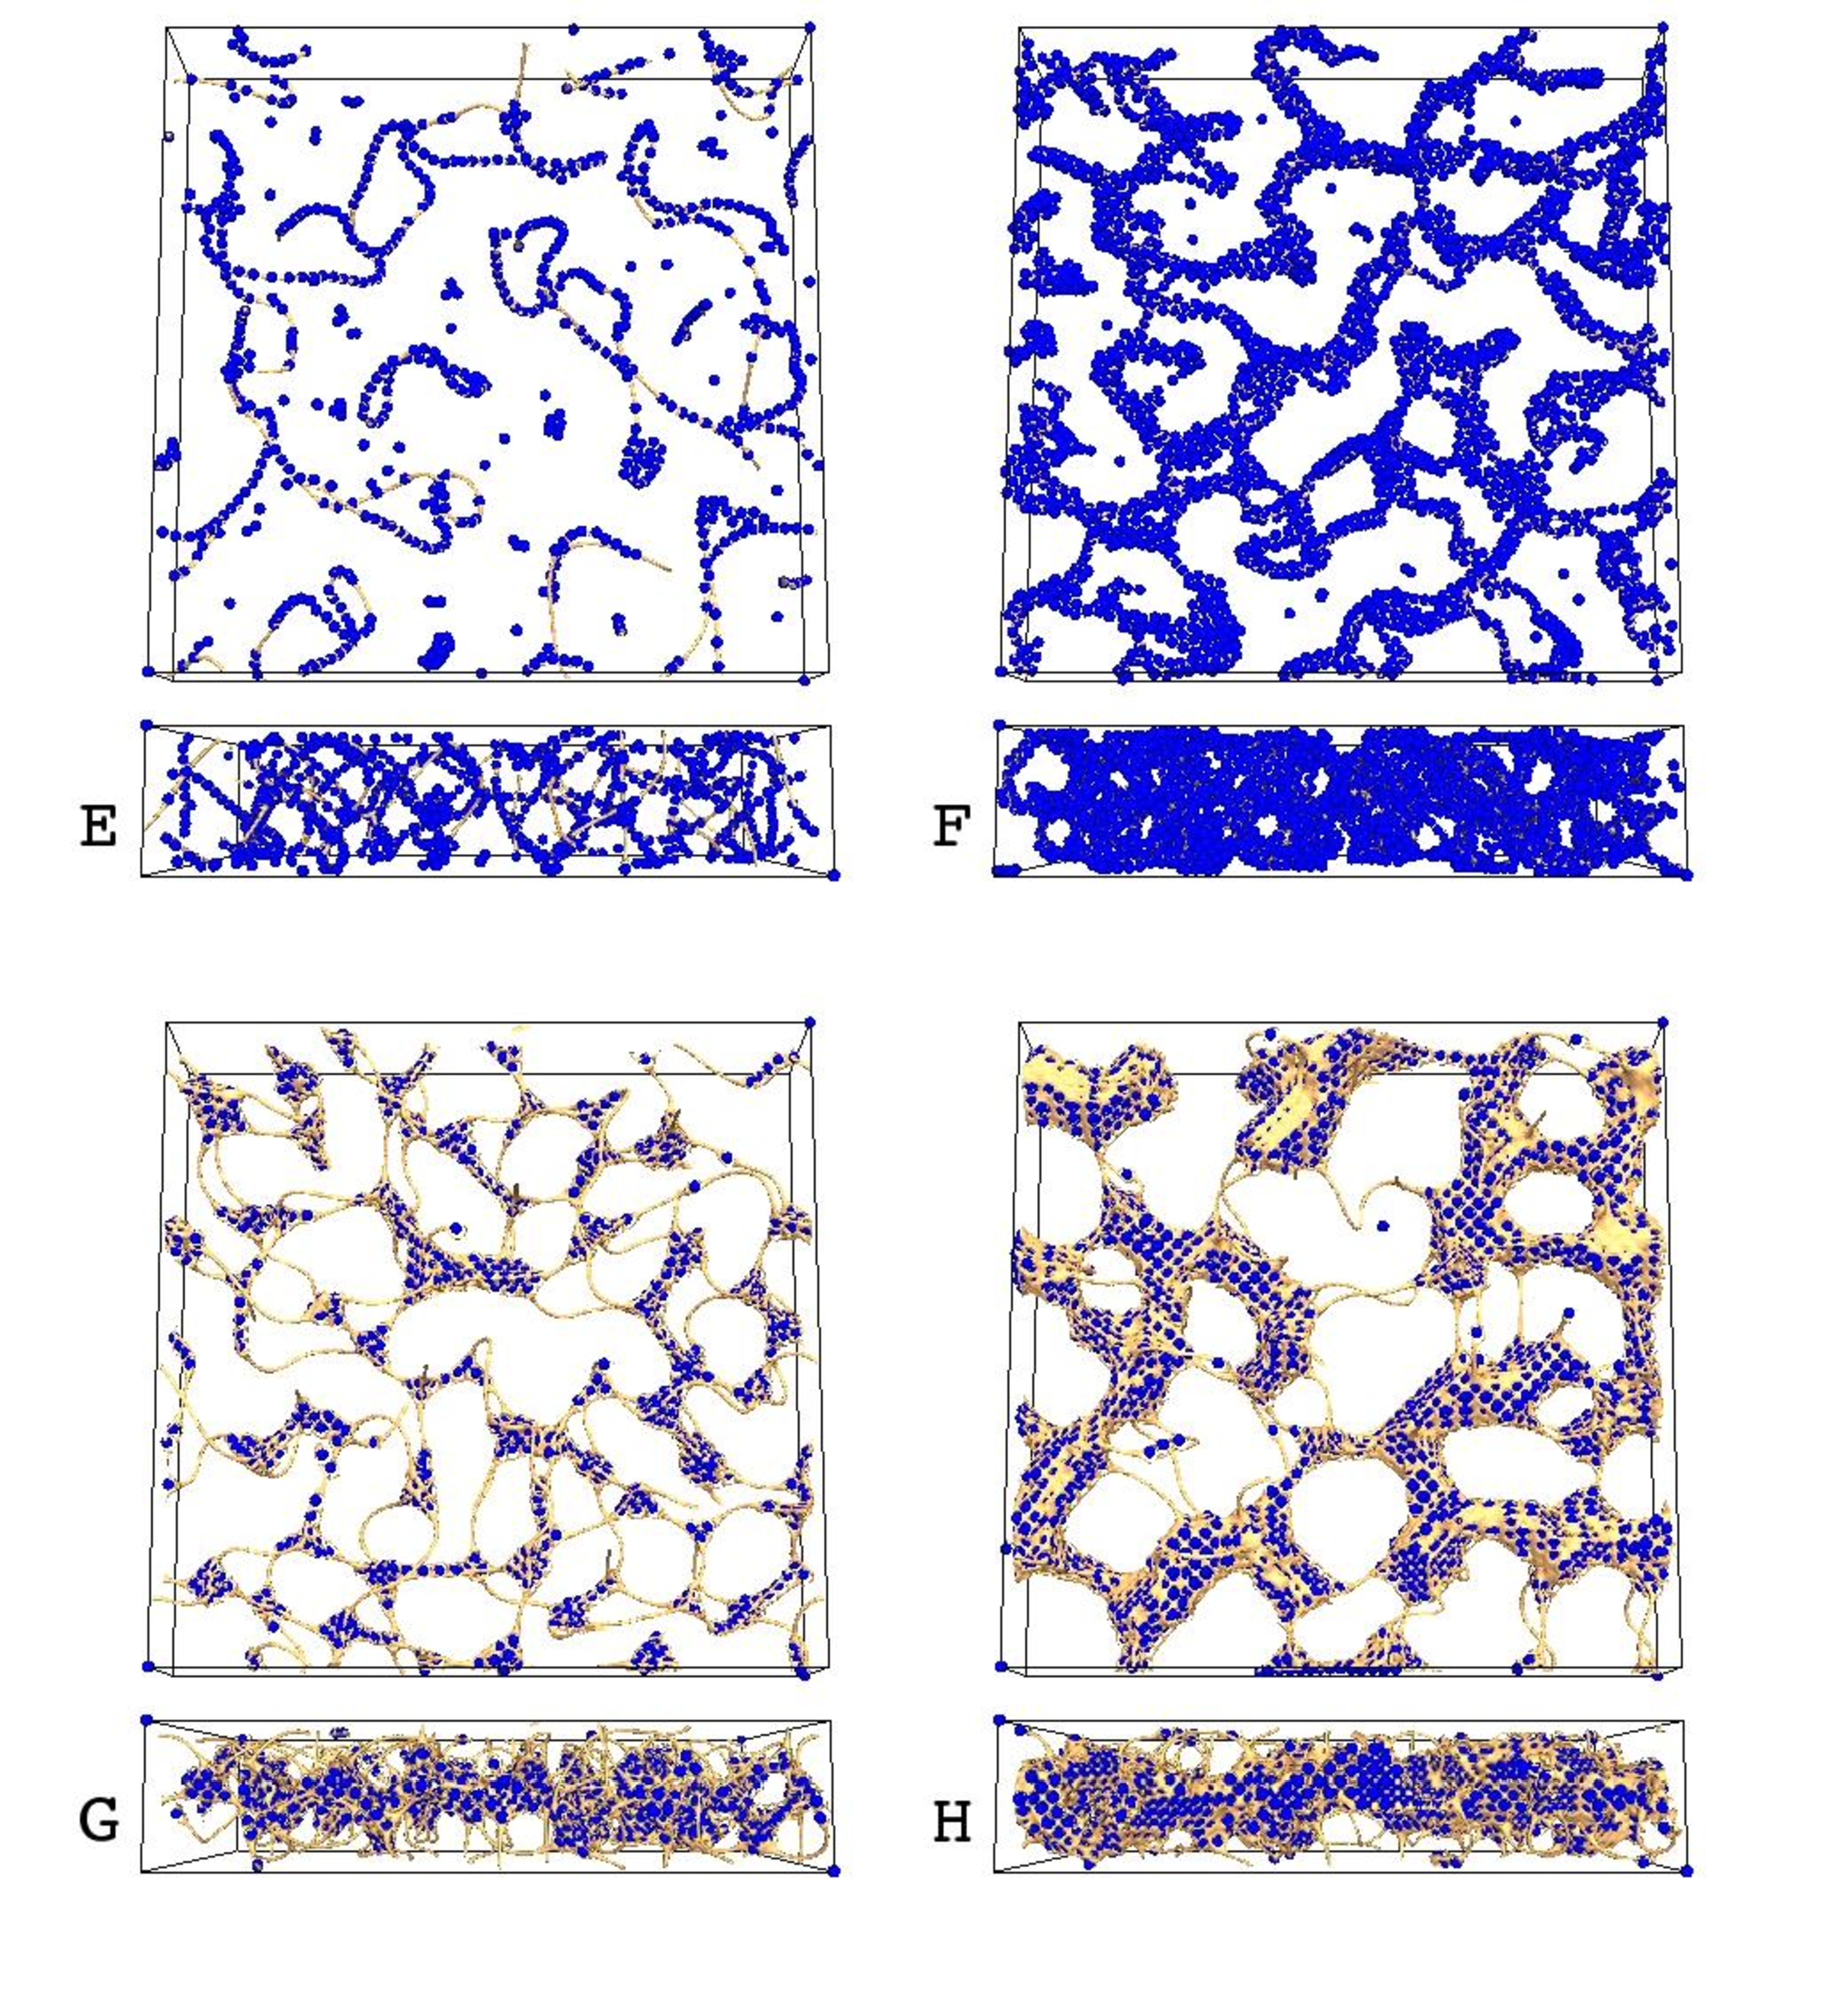
\includegraphics[scale=0.42]{support-fig6.pdf}
\end{center}
\caption{\textbf{Confined blue phase structures.}
As for main manuscript Fig.~2 E--H (confined geometry with planar
anchoring walls at both top and bottom), but for the entire simulation
system of 256$^2\times$56 lattice sites. Each shows a top view and
side view of the same simulation state. (E) colloid solid volume fraction 1\%
and weak anchoring; (F) 4\% solid volume fraction and weak anchoring;
(G) 1\% solid volume fraction and strong anchoring; (H) 4\% solid
volume fraction and strong anchoring.}
\end{figure}

\newpage


\begin{figure}[!h]
\begin{center}
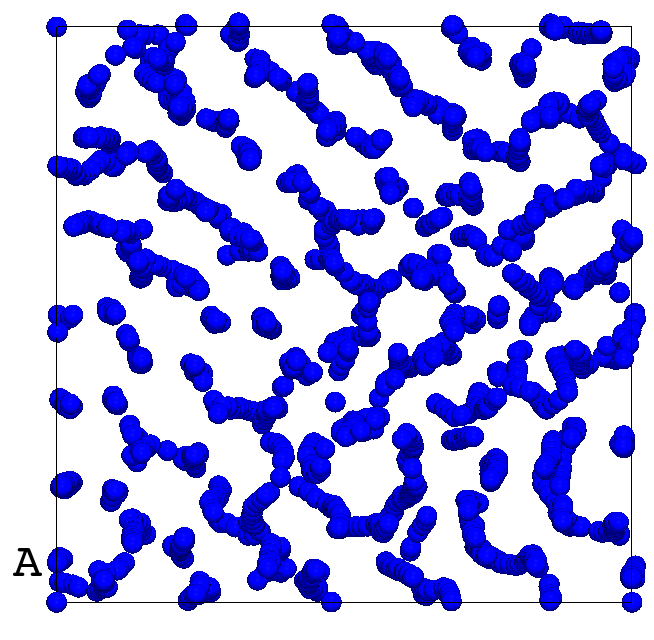
\includegraphics[width=0.34\columnwidth]{col_parallel_x_run1341.png}
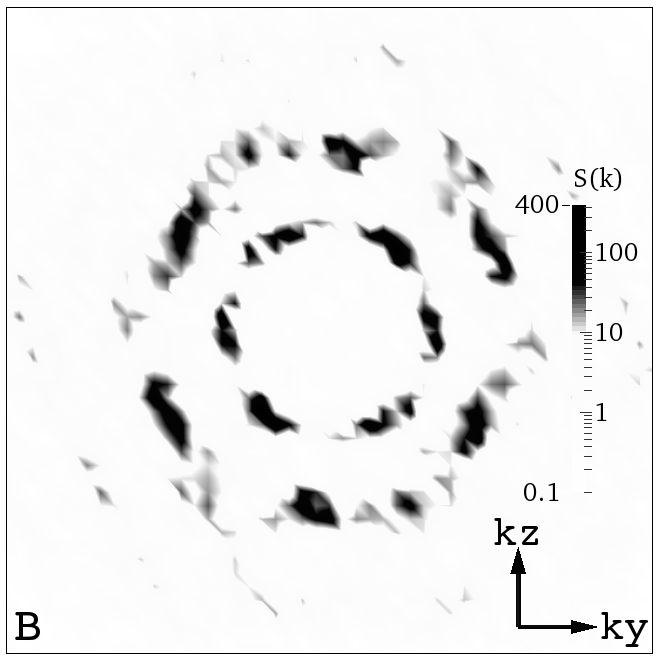
\includegraphics[width=0.32\columnwidth]{sq_x_run1341_2.png}
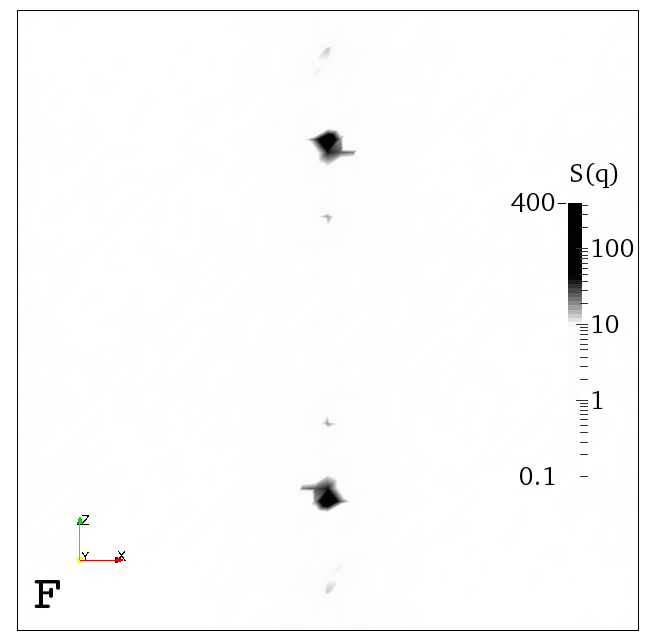
\includegraphics[width=0.32\columnwidth]{sq_y_run1341.png}
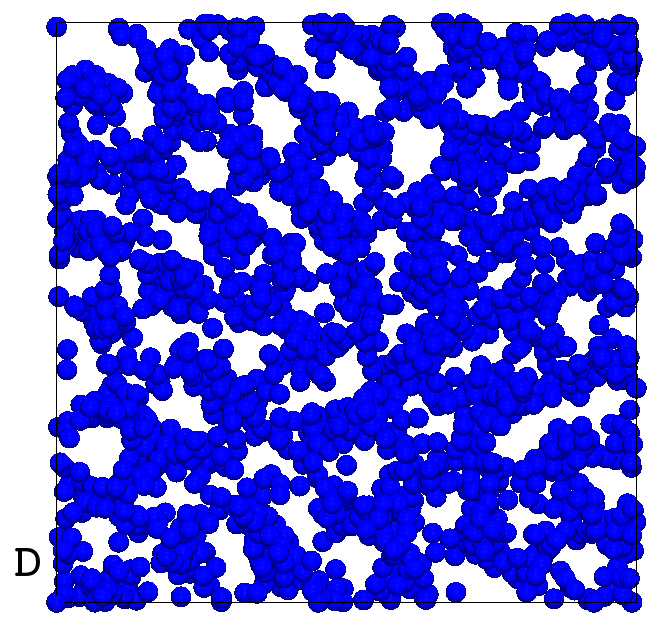
\includegraphics[width=0.34\columnwidth]{col_parallel_x_run1342.png}
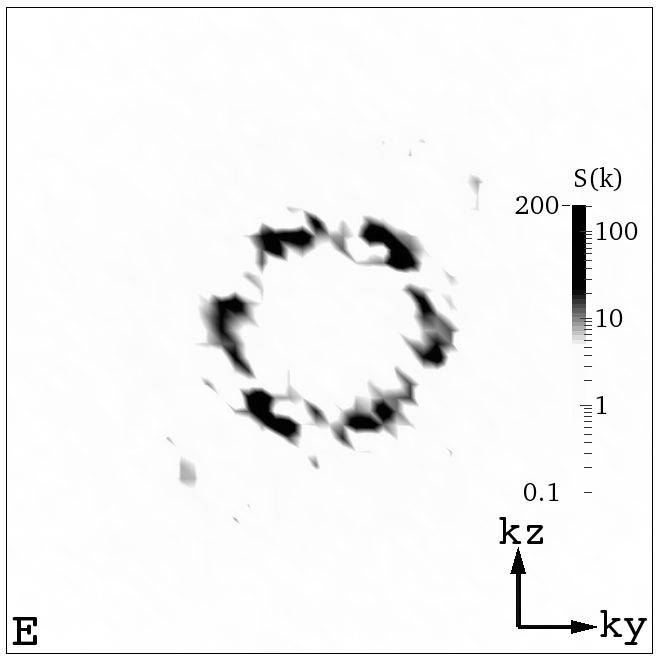
\includegraphics[width=0.32\columnwidth]{sq_x_run1342.png}
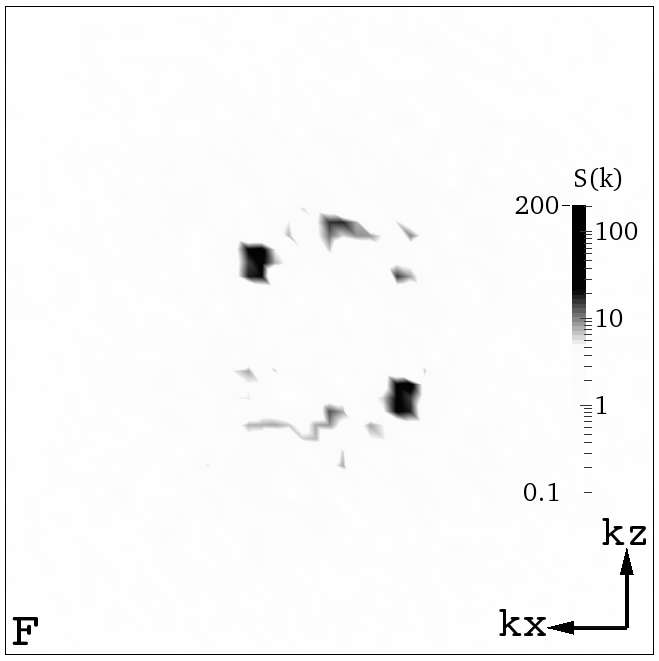
\includegraphics[width=0.32\columnwidth]{sq_y_run1342.png}
\end{center}
\caption{\textbf{Structure with and without electric field.}
(Disclination lines are 
removed for clarity.) Panels A and B reproduce the results in Fig. 3C and
Fig. 3D respectively with the applied field in the $x$-direction 
(out of the plane of the paper). Also included is a cut of the structure 
factor with $k_y = 0$ (panel C). 
Panels D, E, and F show the corresponding situation after the
external field has been removed and the structure allowed to relax,
and show residual hexagonal ordering. The structure factor data is for wave
vectors $k_x = 0; (k_y, k_z) \in [-3\pi/8 , 3\pi/8]$ (panels B and E) and
$k_y = 0; (k_x, k_z) \in [-3\pi/8, 3\pi/8]$ (panels C and F).}
\end{figure}

\newpage

\begin{figure}[!h]
\begin{center}
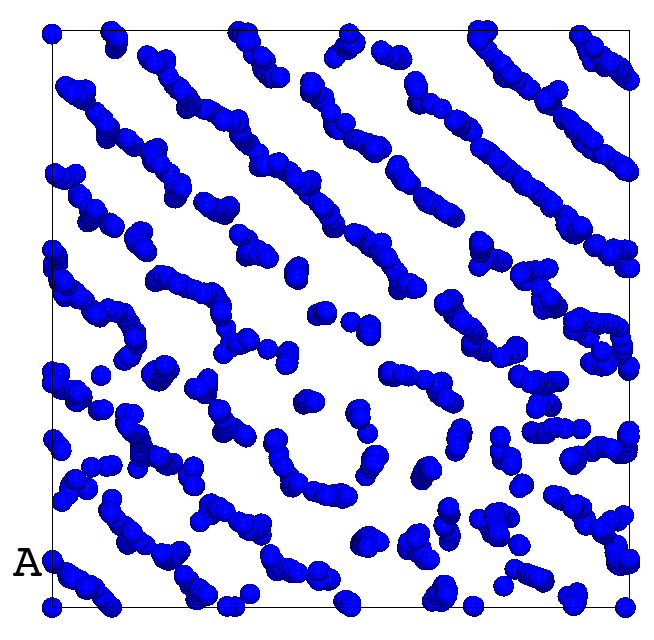
\includegraphics[width=0.34\columnwidth]{col_parallel_y_run1343.png}
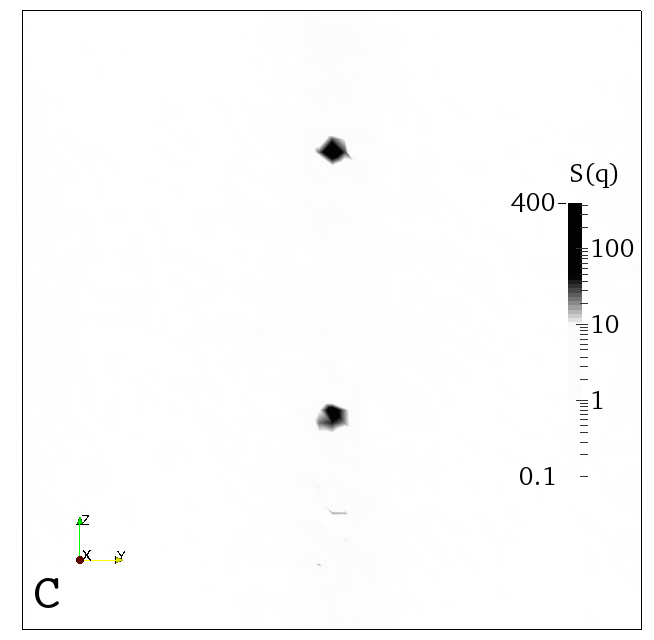
\includegraphics[width=0.32\columnwidth]{sq_x_run1343.png}
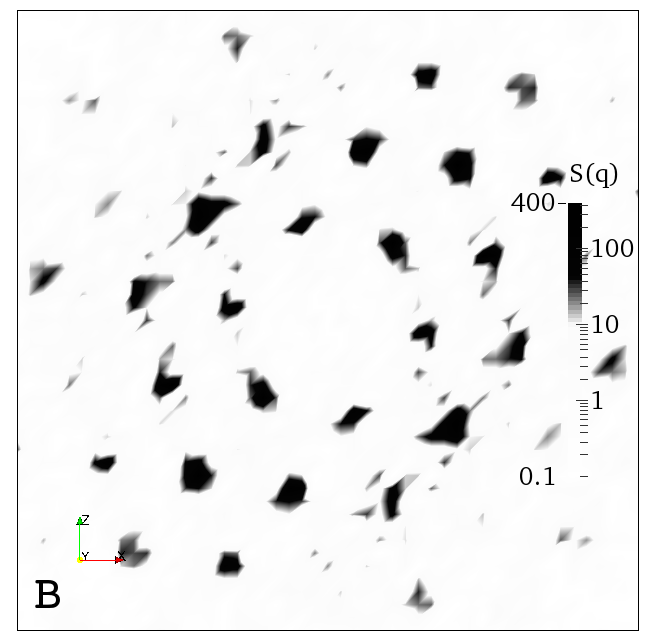
\includegraphics[width=0.32\columnwidth]{sq_y_run1343.png}\\
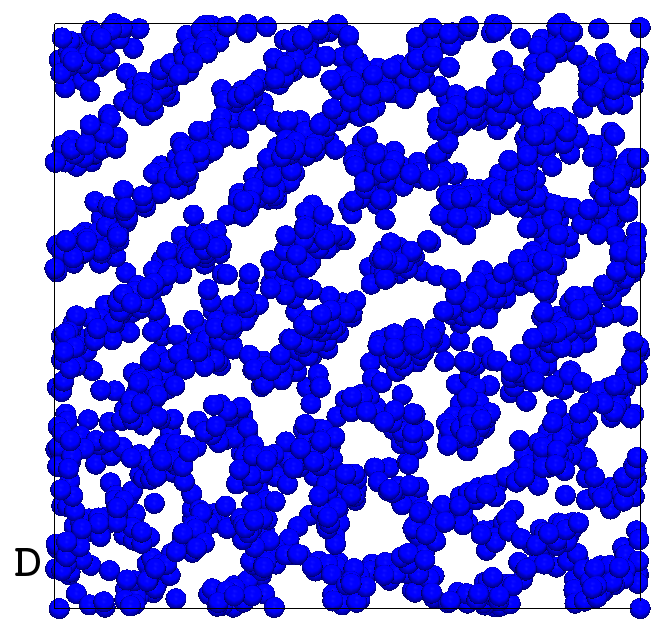
\includegraphics[width=0.34\columnwidth]{col_parallel_y_run1344.png}
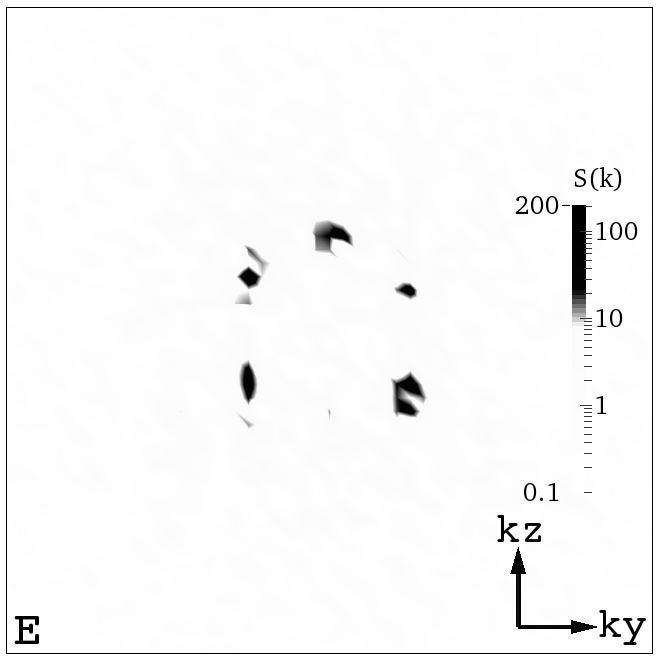
\includegraphics[width=0.32\columnwidth]{sq_x_run1344.png}
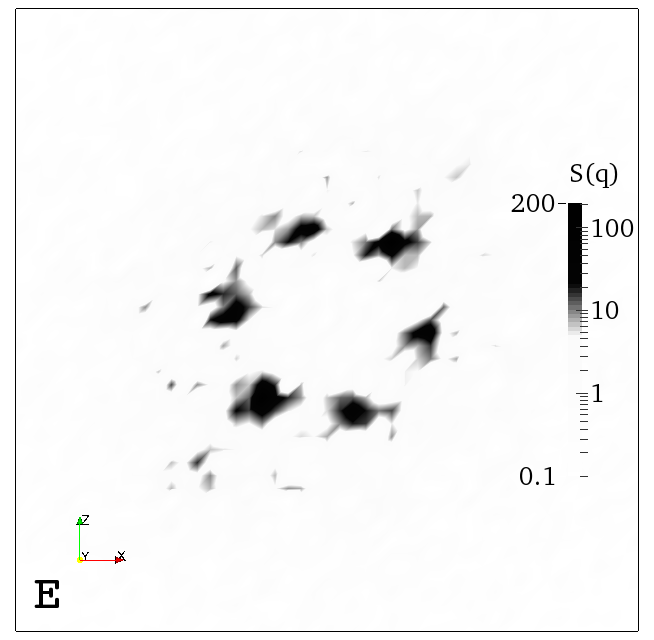
\includegraphics[width=0.32\columnwidth]{sq_y_run1344.png}\\
\end{center}
\caption{\textbf{Cycling the electric field.}
Starting from the final position of
Supplementary Fig.~7 panel~D, the field is re-applied, this time in the
$y$-direction. The corresponding view of the particle distribution is
shown, again viewing along the field direction, in panel A.
Corresponding structure factor cuts with $k_x = 0$ and $k_y = 0$ are
shown in panels B and C, respectively. The corresponding situation when
the field is again switched off, and the structure allowed to relax,
is shown in panels D, E, and F. The wave vector values used are the
same as in Supplementary Fig.~7.}
\end{figure}

\newpage

\begin{figure}[!h]
\begin{center}
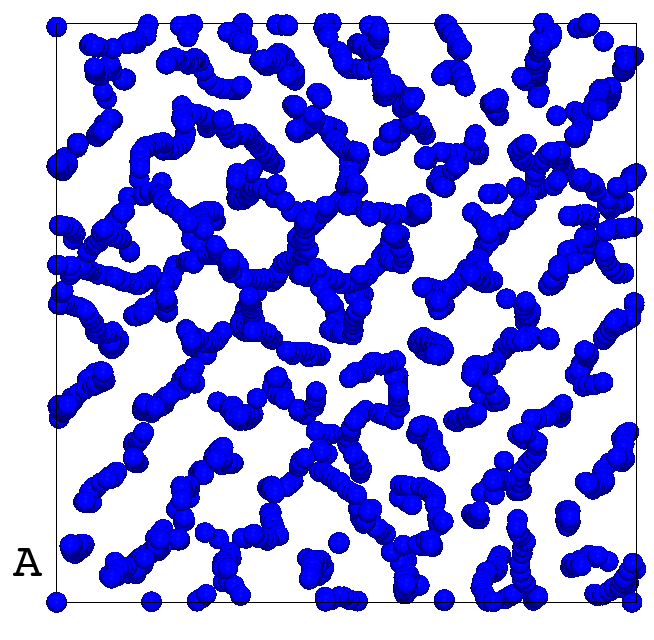
\includegraphics[width=0.34\columnwidth]{col_parallel_x_run1345.png}
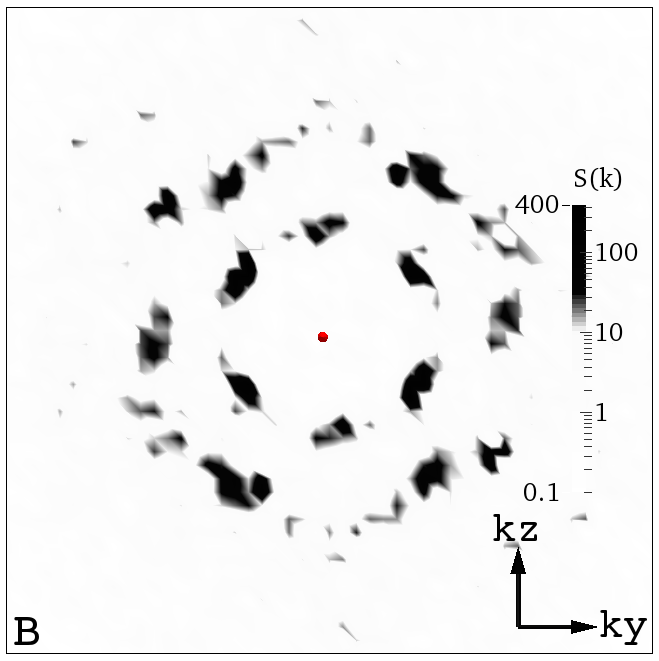
\includegraphics[width=0.32\columnwidth]{sq_x_run1345.png}
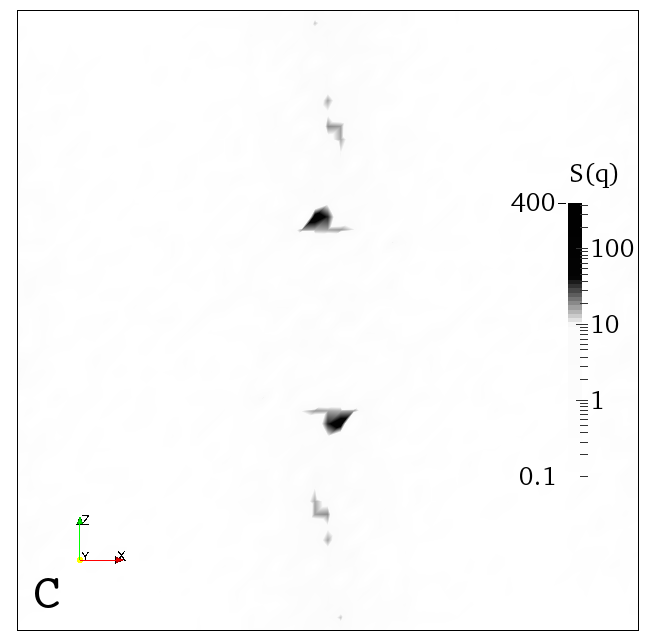
\includegraphics[width=0.32\columnwidth]{sq_y_run1345.png}\\
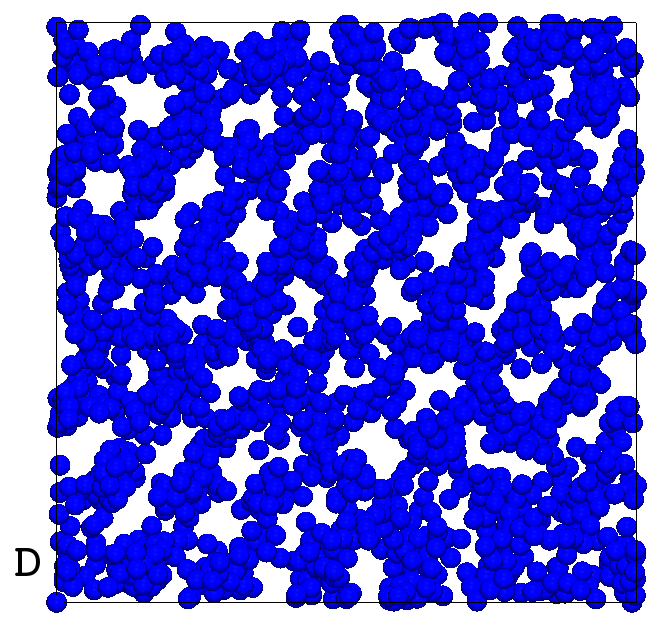
\includegraphics[width=0.34\columnwidth]{col_parallel_x_run1347.png}
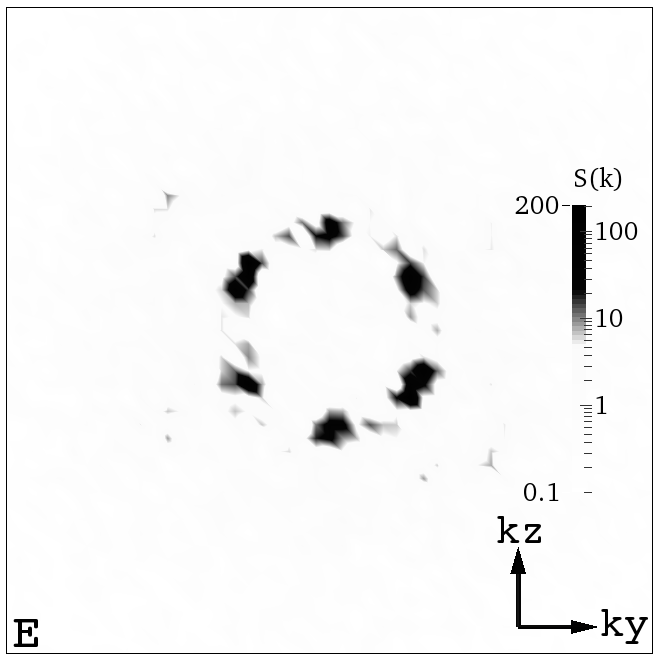
\includegraphics[width=0.32\columnwidth]{sq_x_run1347.png}
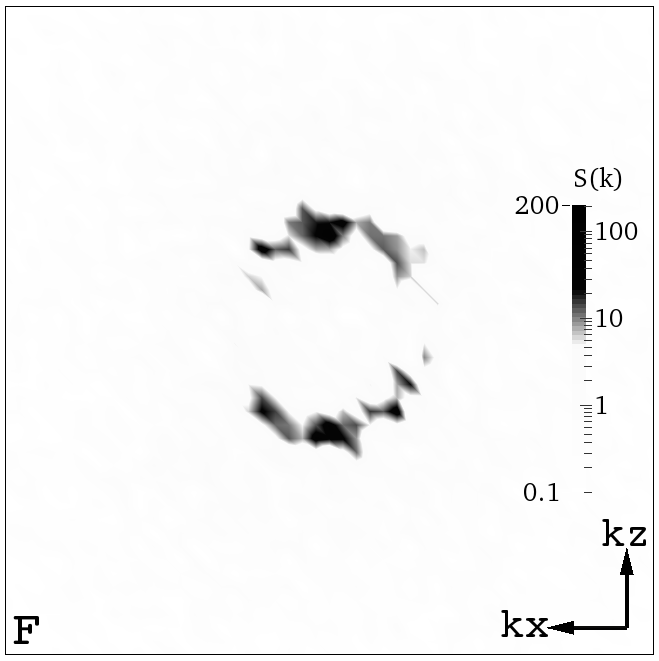
\includegraphics[width=0.32\columnwidth]{sq_y_run1347.png}
\end{center}
\caption{\textbf{Cycling the electric field further.}
Starting from the final
position of Supplementary Fig.~8 panel~D, the field is re-applied
again in the $x-$direction. Panel A shows the particle configuration
viewed along the field direction, and panels B and C show the structure
factor with $k_x = 0$ and $k_y = 0$ respectively. The corresponding
situation when the field is removed and the structure allowed to relax
is shown in panels D, E, and F. The wave vector values are again as
in Supplementary Fig.~7. Note that the on and off states are 
equivalent to those in Supplementary Fig.~7, up to a rotation.
This is because all hexagonal structures perpendicular to the field
direction are energetically degenerate,
and the actual orientation of the hexagon emerges spontaneously during
switching. }
\end{figure}


\vfill\pagebreak


{\bf Supplementary Table}

\begin{table}[h]
\begin{center}
\begin{tabular}{|l|c|c|c|c|c|c|c|}
\hline
         & $A_0$ & $\gamma$ & $K$ & $p$ & $\kappa$ & $\tau$ & $WR/K$\\
\hline 
Bulk BPI & 0.01 & 3.086 & 0.007061 & 32$\sqrt{2}$ & 0.6902 & -0.2500 &
0.23, 2.3\\
\hline
Bulk Quench & 0.01 & 3.086 & 0.007061 & 32$\sqrt{2}$ & 0.6902 & -0.2500 &
0.23, 2.3 \\
\hline
Confined & 0.01 & 3.086 & 0.01897 & 64 & 0.8 & -0.2500 & 0.23, 2.3\\
\hline
External field & 0.004& 3.086 & 0.02 & 32 & 2.6 & -0.2500 & 0.23\\ 
\hline
\end{tabular}
\end{center}
\caption{\textbf{Free energy parameters used in the simulations.} Bulk BPI
correspond to Fig.~1 (A-D), bulk quench to Fig.~1 (E--H); confined
geometries are shown in Fig.~2; and the external field case is
relevant for Fig.~3.}
\label{table:params}
\end{table}

\vfill
\pagebreak

{\bf Supplementary Methods}

\noindent
\textbf{Parameter details for bulk BPI.}
The parameters for the free energy are chosen to be representative
of blue phase I: chirality $\kappa \sim 0.7$ and reduced temperature
$\tau = -0.25$.
The full free energy parameters are shown in Table~\ref{table:params}.
The order parameter tensor $Q_{\alpha\beta}$ for bulk blue phase I is
initialised from an approximation in high chirality limit
\cite{blue1,oliver1}. Systems of 128$^3$ lattice sites are
used with a pitch length of $p = 32\sqrt{2}$, which accommodates 4$^3$
unit cells with fully periodic boundary conditions.
Simulations at different solid volume fractions (1\% and 4\%), and different 
surface anchoring strengths ($WR/K = 0.23$ and $WR/K = 2.3$) representing
``weak'' and ``strong'' anchoring are run for two million simulation
time steps.
The initial distribution of the colloid positions is set at random
for the required solid volume fraction; the colloids are initially
at rest.

To generate a disordered network of disclination lines, a ``quench''
is performed in which the order parameter is initialised via a
locally chosen random director, and
%Eq.~\ref{eq:surf_q} MAIN TEXT Q_0 = .... 
Eq.~15
employed with a small amplitude $q^0 = 10^{-7}$ to
provide an order parameter.
The mean-field spinodal point at $\gamma = 3.0$ is avoided and
the parameters are the same as for the initial simulations with
pitch $p = 32\sqrt{2}$. The chirality and reduced temperature (see
Table~\ref{table:params}) remain appropriate for BPI.
Colloids are added as before and the simulations run for 2 million
simulation steps.

For simplicity,  the size of the BPI unit cell is not allowed to 
readjust dynamically to minimise free energy (there is no 
``redshift''~\cite{blue1}): this would lead to quantitatively different 
values of the free energy, but qualitatively similar structures. 

\noindent
\textbf{Parameters for confined BPI.}
Here, a narrow sandwich of fluid is placed between flat walls in
perpendicular to the narrow coordinate direction, and with periodic
boundaries in the other two directions. The system size used in all
cases is 256$^2 \times$56 lattice sites. Each simulation is a ``quench''
in a similar manner to that used in the bulk: the order parameter is
initialised randomly. The free energy parameters (see Table~\ref{table:params})
are again appropriate for (equilibrium) blue phase I
(chirality $\kappa = 0.8$ and
reduced temperature $\tau = -0.25$). The cholesteric pitch is set
to be $p = 64$, providing a slightly better resolution than the bulk
simulations.

The surface anchoring for colloids is as before: always normal, but with
$WR/K = 0.23$ and $WR/K = 2.3$. The colloid solid volume fractions are
1\% and 4\%.
For both normal and planar anchoring at the walls,
the strength is adjusted to correspond to that used for the strongly
anchoring particles.
All simulations are run for two million simulation time steps.

\noindent
\textbf{External electric field.}
For the simulations of BPIII with colloidal particles a system size of
$128^3$ is used with a cholesteric pitch of $p=32$ in lattice units. 
The simulations are
performed at chirality $\kappa=2.6$ and reduced temperature $\tau=-0.25$.  
An initial configuration of
randomly oriented and positioned double twist cylinders is used,
from which an amorphous BPIII network emerges \cite{oliver-bp3}. This structure
is equilibrated for $6\times10^{5}$~LB time steps until no significant
further evolution is observed. 

The colloidal particles with weak
normal anchoring ($WR / K= 0.23$), are then inserted with randomly chosen positions,
and the composite system is equilibrated for another $1.2\times10^{6}$
time steps.
At the end of the equilibration phase the uniform electric field
with reduced field strength ${\cal E} = 0.8$ 
is switched on (oriented along the $z$-direction), and the simulation
run for a further $1.2\times10^{6}$ time steps.
This is found to be sufficiently long for a hexagonal structure to
emerge and saturate.
If the electric field is then switched off, and the system quickly relaxes
to a metastable state which shows a residual anisotropy in the
colloidal distribution. The total length of this final relaxation phase
is $1\times10^6$ LB time steps.

\noindent
\textbf{Disclination rendering.}
In all cases visualisation of the defect lines is carried out via
an isosurface of the scalar order parameter~$q$ determined from the
largest eigenvalue of the local order parameter tensor. A low value
of the scalar order parameter~$q$ (typically in the range~0.12--0.14)
unambiguously identifies the disclinations.

\noindent
\textbf{Computation of the structure factor.}
To provide structural information about the field-aligned 
states and the residual anisotropy after switch off a 
procedure similar to the one described in \cite{oliver-bp3} is
followed.
The structure factor $S(\mathbf{k})$ in the current approach is
defined via the Fourier transform of the colloid density $F(\mathbf{k})$:
\begin{equation}
S({\bf k}) =  |F({\bf k})|^2, \mathrm{with}\
F({\bf k}) = \int d^3{\bf r} \rho({\bf r}) e^{i {\bf k. r}}.
\end{equation}
The colloid density $\rho({\bf r})$ is a discretised density and taken to be
$\rho({\bf r})=1$ if a lattice site at ${\bf r}$ is part of a colloid
and $\rho({\bf r})=0$ otherwise. This definition, which deviates from the 
standard definition of a structure factor and does not consider the colloids 
as point-like objects, allows the same structural information
to be obtained in a simple way.

\noindent
\textbf{Parameter mapping to physical units.}
To get from simulation to physical units, a calibration of scales of
length, energy and time in the simulations is required. For similar
mappings see,
e.g.~\cite{denniston2}.

The length scale can be set by mapping the half pitch to a realistic blue
phase unit cell size, which is in the 100--500~nm range \cite{blue1}. 
For bulk simulations (Fig.~1 and Fig.~3 in the main text), a suitable choice
is one where one simulation unit (lattice site) corresponds to 10~nm. Therefore
the colloidal size in Figs.~1 and~3 corresponds to $\sim$ 50~nm. 

To obtain an energy scale, it is possible to choose $A_0 \simeq 10^6$~Pa,
which is reasonable following Ref.~\cite{blue1} (this is also the choice in
Ref.~\cite{oliver2}). This choice leads to a simulation unit of
free energy (or stress) equal to $10^{8}$~Pa in Figs.~1 and~3.
From the energy and length scales one can map elastic constants to
physical units: for instance, the simulation in Fig.~1 corresponds to
a liquid crystal with splay, bend and twist (Frank) elastic constants
equal to 35 pN (or equivalently $K=70$~pN).

The timescale calibration may be obtained from (see e.g.~\cite{denniston})
\begin{equation}
\gamma_1=\frac{2q^2}{\mathit{\Gamma}},
\end{equation}
which relates the rotational viscosity $\gamma_1$ to the ordering strength
$q$ and the order parameter mobility $\mathit{\Gamma}$.
In the present simulations, $\mathit{\Gamma} = 0.5$ and the value of $\gamma$
for the simulation in Fig.~1 leads to $q=1/2$.   
For real liquid crystalline materials, $\gamma_1$ usually lies in range
$10^{-2}-1$ Pa s~\cite{deGennes}; for definiteness say
$\gamma_1 = 1$~Pa~s (equivalently 10 poise). Given the previous mapping for
free energy (or stress) units, this leads to a simulation unit of time equal
to $10^{-8}$~s. The total simulated time in Figs. 1-3 is therefore in the
millisecond range. 

To calibrate the electric field strength 
one can equate the value of the dimensionless parameter ${\cal E}$ in the 
simulations with that of a hypothetical experiment.
Given the previous value for $A_0$, and a dielectric anisotropy of 20
(or equivalently $\epsilon_\mathrm{a}=20\epsilon_0$, with $\epsilon_0$ the
dielectric permittivity of vacuum), an electric field
of 100 V~$\mu$m$^{-1}$ is obtained. This corresponds to a value of
${\cal E}\sim 0.4$ (considering a value of $\gamma=3.0857$ as in
Fig.~3 of the main text).

Given these mappings, all quantities can be easily transformed from
simulation to physical units and vice versa. For example Figs.~1 and~2
use an isotropic viscosity $\eta \simeq$~0.01 and~0.1 in simulation units,
which translate into $0.01-0.1$~Pa~s respectively. This is sensible (if 
slightly low) for a molecular nematogen in the isotropic phase. 
The effective viscosity in ordered phases is higher, but this is ensured
in our model by the coupling to the order parameter.
Note that the density is set to unity in the simulations: this
corresponds to a fluid density which is about a thousand times larger
than in experiments. This makes no difference in practice as
the Reynolds number $= \rho V\Lambda/\eta$ (where $V$ is a typical
velocity, in our simulations around $10^{-5}$ in lattice units, 
and $\Lambda$ is a typical length scale, e.g. the size of a unit cell) 
remains small enough~\cite{codef}. 

To summarise, the simulations represent BP-forming materials, with the
interpretation of the simulation units for length, time, and energy
density being close to 10~nm, 10~ns, and 100~MPa respectively.
For a Frank eleastic
constant of $K = 70$~pN and unit cell sizes in the range
$\lambda =$100--500~nm, a corresponding shear modulus $G \simeq
K/\lambda^2 =$ 0.3--7~kPa.

\vfill
\pagebreak


\begin{thebibliography}{99}

\bibitem{blue1}
Wright, D.C., and Mermin, N.D.,
Crystalline liquids: the blue phases,
{\it Rev. Mod. Phys.} {\bf 61,} 385-432 (1989).
\bibitem{oliver1}
Henrich, O., Marenduzzo, D., Stratford, K., and Cates, M.E.,
Thermodynamics of blue phases in electric fields,
\textit{Phys. Rev. E}, \textbf{81} 031706 (2010).
\bibitem{oliver-bp3}
Henrich, O., Stratford, K., Cates, M.E., and Marenduzzo, D.,
Structure of blue phase III of cholesteric liquid crystals,
{\it Phys. Rev. Lett.} {\bf 106}, 107802 (2011).
\bibitem{denniston2}
Denniston, C., Marenduzzo, D., Orlandini, E., and  Yeomans, J.M.,
Lattice Boltzmann algorithm for three-dimensional liquid-crystal
hydrodynamics,
\textit{Philos. Trans. R. Soc. London, Ser. A} \textbf{362}, 1745 (2004).
\bibitem{oliver2}
Henrich, O., Stratford, K.,  Marenduzzo, D., and Cates, M.E.,
Ordering dynamics of blue phases entails kinetic stabilization of
amorphous networks, 
\textit{Proc. Acad. Sci. USA} \textbf{107}, 1312 (2010).
\bibitem{denniston}
Denniston, C., Orlandini, E., and Yeomans, J.M.,
Lattice Boltzmann simulattions of liquid crystal hydrodynamics,
\textit{Phys. Rev. E} \textbf{63}, 056702 (2001).
\bibitem{deGennes}
de Gennes, P.-G., and  Prost, J.,
{\it The Physics of Liquid Crystals} (Clarendon Press, 1995).
%\bibitem{fournier2005}
%J.-B. Fournier and P. Galatola,
%\textit{Europhys. Lett.} \textbf{72}, 403 (2005).
\bibitem{codef} Cates, M.E.,  et al.,
Simulating colloid hydrodynamics with lattice Boltzmann,
\textit{J. Phys. Condens. Matter} \textbf{16},  3903 (2004). 


\end{thebibliography}

%\newpage
\clearpage
 
%{\bf Captions for Supplementary Movies} \\
%
%{\bf Supplementary Movie 1:} 
%The final state of the simulation as shown in Fig.~1A. The movie
%rotates the configuration to reveal more clearly its structure.\\

%{\bf Supplementary Movie 2:} 
%The final state of the simulation as shown in Fig.~1B. The movie
%rotates the configuration to reveal more clearly its structure.\\


%{\bf Supplementary Movie 3:} 
%The final state of the simulation as shown in Fig.~1C. The movie
%rotates the configuration to reveal more clearly its structure.\\


%{\bf Supplementary Movie 4:} 
%The final state of the simulation as shown in Fig.~1D. The movie
%rotates the configuration to reveal more clearly its structure.\\


%{\bf Supplementary Movie 5:} 
%The configuration after the initial relaxation phase in Fig.~3. The movie
%shows a rotation of the configuration. The distribution of the colloidal
%particles is isotropic, with the particles forming clusters and having a
%tendency to occupy positions at the intersection of the BPIII disclination
%lines.\\

%{\bf Supplementary Movie 6:} 
%Configuration in a homogeneous electric field with strength
%corresponding to ${\cal E}=0.8$. The movie
%shows a rotation of the configuration.
%A hexagonal pattern emerges where the particles form chains
%situated at the vertices of the honeycomb-like structure. \\

\end{document}
